\section{TECHNICAL APPROACH}
We propose a recognition algorithm based on DTW and
decision fusion. The flowchart of the algorithm is shown in
Fig. 2.

\begin{figure}[t]
\centering
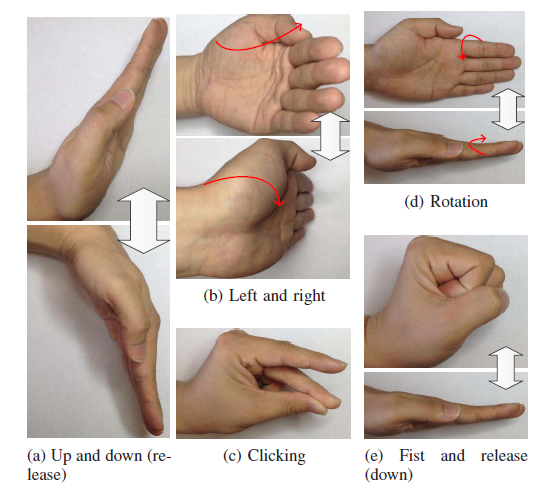
\includegraphics[width=8cm]{fig/fig3}
\caption{Gestures set. (No distinction between the down gesture
from the up position and the release gesture from the fist
position.)}
\end{figure}

\begin{figure}[t]
\centering
\includegraphics[width=8cm]{fig/fig4}
\caption{Filtered Signal}
\end{figure}

\subsection{Gesture Set}
Fig. 3 shows the tested gestures. What distinguishes them
from those that can be handled by previous ACC-based systems
\cite{c4}, \cite{c13}, \cite{c14} is their use of significant wrist movements,
such as hand up, clicking, and making a fist.

\subsection{Preprocessing and Segmentation}
In the preprocessing stage, a median filter is used for
both MTS and ACC to remove the high-frequency noise. A
high-pass filter (HPF) is then used to remove the gravity
factor in all three axes of ACC. After the filtering, only the
MTS signal is normalized to reduce the influence of signal
amplitude variation due to different speeds of performing the
same gesture. The raw and the filtered signals are shown in
Fig. 4.

Segmentation is based solely on the amplitude of the MTS
signal. A double-thresholding algorithm, as shown in Algorithm
1, runs point by point to divide the signal into segments.
Previous single ACC-based systems \cite{c13}, \cite{c14} usually use a
fixed-size sliding window with overlap to segment the signal.
The signal content within the window has to be checked
constantly to see if any valid gestures exist. Longer delay will
be caused by the fixed window size. By setting the starting
point and ending point in the signal of interest, our MTS-based
segmentation improves the system response time while
naturally rejecting some segments based on their length. Any
signal that is too short or too long will be automatically
discarded and will not go to the computationally complex
dynamic programming.

The algorithm keeps counting the samples across or below
the corresponding amplitude threshold. Based on a series of
counting conditions, the algorithm resets the counter or outputs
the starting and ending points of the given segment. Fig. 5
shows a segmented MTS signal with its starting and ending
points. This algorithm requires that the gestures be done
separately with enough resting interval. Otherwise, several
segments may be counted as one and may be discarded due to
oversize.

\begin{figure}[t]
\centering
\includegraphics[width=8cm]{fig/fig5}
\caption{Signal Segmentation}
\end{figure}

\subsection{Dynamic Time Warping Algorithm}
As shown in Fig. 2, DTW is the core algorithm of detection.
It is performed to both MTS and ACC signals. After
preprocessing and segmentation, MTS signal is first checked
with all stored templates using one-dimensional DTW. Only
those templates with sufficiently high scores can be sent to
the next step. If the segmented signal does not match any
pattern over the threshold, then it will be discarded. We find
this rejection step to be able to effectively reduce the number of
false-positive detections due to casual, unintended movement.
The basic DTW algorithm is shown in Algorithm 2.

DTW finds a match between two time sequences by dynamic
programming. The idea is to find the shortest path in the
cost matrix as shown in Fig. 6, where each cell represents the
similarity score between the two corresponding subsequences.
The distance between two MTS samples is just the absolute
value, while for 3D acceleration samples, the distance is
calculated based on Euclidean distance as in shown in Eq. (1).
The matched signals in all four dimensions are shown in Fig. 7.

\begin{tiny}
\begin{equation}
\sqrt{(ACCX_1 - ACCX_2)^2 + (ACCY_1 - ACCY_2)^2 + (ACCZ_1 - ACCZ_2)^2}
\end{equation}
\end{tiny}

Two constraints are implemented here: warping window
constraint and slope constraint \cite{c11}. Warping window constraint
(line 1) prevents one point from matching any point
too far away by setting global forbidden area, shown as the
gray cells in Fig. 6, to eliminate the path far off the diagonal.
The local slope constraint (line 2) avoids the alignment paths
that are too steep or too shallow as shown in Fig. 6. The
slope value along the optimal path from the starting point to
each cell is stored in separate slope matrices. When exceeding
the threshold, the path will be discarded along the way. The
slope matrix is updated on line 3. If the two sequences are too
different from each other, then the template sequence will be
automatically rejected before DTW.
\subsection{Decision Fusion}
The final matching score of the segmented signal to each
template is given by Formula (2). It is a weighted average
of both MTS and ACC scores with the weight $\gamma$ = 0.66. The
template with the best score is selected as the output gesture.

\begin{small}
\begin{equation}
score\_final = \gamma\cdot score\_ACC+(1-\gamma)\cdot score\_MTS
\end{equation}
\end{small}